%
%  Chris Thoma
%
\documentclass[12pt,fullpage]{article}
\usepackage{fullpage}
\usepackage{psfrag}                                          % LaTeX graphics tool
\usepackage{pslatex}                                         % avoids the default cmr font
\usepackage{graphicx}                                        % graphics package 
\usepackage{epsfig}                                          % figures
\usepackage{hyperref}
\usepackage{color}

\begin{document}

\noindent
{\bf Poisson distribution} (from \color{blue}\url{http://www.math.wm.edu/~leemis/chart/UDR/UDR.html}\color{black})

\noindent
The shorthand $X \sim {\rm Poisson}(\mu)$ is used to indicate that the
random variable $X$ has the Poisson distribution with positive parameter $\mu$.
A Poisson random variable $X$ with scale parameter $\mu$ has probability mass function 
$$
f(x) = \frac{\mu ^ {\kern 0.08 em x} e ^ {-\mu}} {x!} \qquad \qquad x = 0,1,2 , \ldots \,.
$$
The Poisson distribution can be used to model the number of events in an interval associated
with a process that evolves randomly over space or time.
Applications include the number of potholes over a stretch of highway, the number of typographical errors
in a book, the number of customer arrivals in an hour, and the number of earthquakes in a decade.
The Poisson distribution can also be used to approximate the binomial distribution when $n$ is
large and $p$ is small.
The probability mass function with $\mu = 8.56$ is illustrated below.
{\begin{figure}[h!]
\begin{center}
\psfrag{labx}{$x$}
\psfrag{labf}{$f(x)$}
\includegraphics[width=3.2in]{PoissonPlot.ps}
\end{center}
\end{figure}}

\noindent
The cumulative distribution function on
the support of $X$ is
$$
F(x) = P(X \le x) = \frac{\Gamma(x + 1,\  \mu)}{\Gamma(x + 1)} \qquad \qquad x = 0,1,2 , \ldots \,.
$$
The survivor function on the support of $X$ is
$$
S(x) = P(X \ge x) = \frac{\Gamma(x + 1) - x \Gamma(x,\ \mu)}{x!} \qquad \qquad x = 0,1,2 , \ldots \,.
$$
The hazard function on the support of $X$ is
$$
h(x) = \frac{f(x)} {S(x)} = \frac{\mu ^ {\kern 0.08 em x} e ^ {-\mu}}{\Gamma(x + 1) - x \Gamma(x,\  \mu)} \qquad \qquad x = 0,1,2 , \ldots \,.
$$
The cumulative hazard function on the support of $X$ is
$$
H(x) = - \ln S(x) = -\ln \left[ \frac{\Gamma(x+1) - x \Gamma(x,\  \mu)}{x!} \right] \qquad \qquad x = 0,1,2 , \ldots \,.
$$
The inverse distribution function of $X$ is mathematically intractable but can run in APPL with statement at the bottom of the page.\\
\\
The median, $m$, of $X$ is approximately (see Wikipedia site)
$$
m \approx \left\lfloor \mu + 1 / 3 - 0.02/ \mu \right\rfloor.
$$
The moment generating function of $X$ is
$$
M(t) = E\left[ e ^ {tX} \right] = e ^ {\kern 0.08em \mu \kern 0.08 em (e ^ t - 1)} \qquad \qquad - \infty < t < \infty
$$
The characteristic function of $X$ is
$$
\phi(t) = E\left[ e ^ {itX} \right] =  e^{\kern 0.08em \mu\kern 0.08 em (e^{it} -1)} \qquad \qquad - \infty < t < \infty
$$
The population mean, variance, skewness, and kurtosis of $X$ are
$$
E[X] = \mu \qquad \qquad 
V[X] = \mu \qquad \qquad 
E\left[ \left( \frac{X - \mu}{\sigma} \right) ^ 3 \right] = \mu ^{-1/2} \qquad \qquad
E\left[ \left( \frac{X - \mu}{\sigma} \right) ^ 4 \right] = 3 + \mu ^{-1}.
$$
%For $X_1, \, X_2, \, \ldots , \, X_n$ mutually independent Poisson($\mu$) random variables,
%the maximum likelihood estimator for $\mu$ is
%$$
%\hat \mu = \frac{1} {n} \sum_{i\, = \,1} ^ n X_i.
%$$
%For $X_1, \, X_2, \, \ldots , \, X_n$ mutually independent Poisson($\mu$) random variables,
%an approximate ${(1 - \alpha) \cdot 100}$\% confidence interval for $\mu$ is 
%$$
%\frac{\hat{\mu} \kern 0.08 em \chi_{2r, \, 1 - \alpha / 2} ^ 2}{2r} < \mu < \frac{\hat{\mu} \kern 0.08 em \chi_{2r, \, \alpha / 2} ^ 2}{2r},
%$$
%where $\chi^2_{2r, \, \alpha / 2}$ is the $1 - \alpha / 2$ percentile of the chi square distribution 
%with $2r$ degrees of freedom.

\vspace{0.1in}

\noindent
{\bf APPL verification:}
The APPL statements
\begin{verbatim}
X := PoissonRV(mu);
CDF(X);
SF(X);
HF(X);
CHF(X);
IDF(X);
Mean(X);
Variance(X);
Skewness(X);
Kurtosis(X);
MGF(X);
\end{verbatim}
verify the cumulative distribution function, survivor function, hazard function, cumulative hazard function,  inverse distribution function, population mean, variance, skewness, kurtosis, and moment generating function.

\end{document}
